\chapter{循环}

\section{自增/自减运算符}

\subsection{自增/自减运算符}

单目运算符中自增++和自减--运算符可以将变量的值加1和减1,但是++和--可以出现在变量之前或之后,即有四种情况:

\begin{enumerate}
	\item 前缀自增
	\item 前缀自减
	\item 后缀自增
	\item 后缀自减
\end{enumerate}

\begin{table}[H]
	\centering
	\setlength{\tabcolsep}{5mm}{
		\begin{tabular}{|c|l|}
			\hline
			\textbf{表达式} & \textbf{含义}        \\
			\hline
			count++         & 执行完所在语句后自增 \\
			\hline
			++count         & 执行所在语句前自增   \\
			\hline
			count--         & 执行完所在语句后自减 \\
			\hline
			--count         & 执行所在语句前自减   \\
			\hline
		\end{tabular}
	}
	\caption{自增/自减运算符}
\end{table}

\newpage

\section{while}

\subsection{while}

在while循环中,当条件满足时重复循环体内的语句。如果条件永远为真,循环会永无止境的进行下去(死循环),因此循环体内要有改变条件的机会。 \\

控制循环次数的方法就是设置循环变量:初值、判断、更新。 \\

while循环的特点是先判断、再执行,所以循环体有可能会进入一次或多次,也有可能一次也不会进入。

\vspace{-0.5cm}

\begin{lstlisting}[language=Java]
while(条件) {
    // code
}
\end{lstlisting}

\vspace{0.5cm}

\mybox{计算5个人的平均身高}

\begin{lstlisting}[language=Java]
import java.util.Scanner;

public class Height {
    public static void main(String[] args) {
        Scanner scanner = new Scanner(System.in);
        double height;
        double total = 0;
        double average;
        int i = 1;
        
        while(i <= 5) {
            System.out.print("输入第" + i + "个人的身高:");
            height = scanner.nextDouble();
            total += height;
            i++;
        }
        
        average = total / 5;
        System.out.println(String.format("平均身高:%.2f", average));
        scanner.close();
    }
}
\end{lstlisting}

\begin{tcolorbox}
	\mybox{运行结果}
	\begin{verbatim}
输入第1个人的身高:160.8
输入第2个人的身高:175.2
输入第3个人的身高:171.2
输入第4个人的身高:181.3
输入第5个人的身高:164
平均身高:170.5
    \end{verbatim}
\end{tcolorbox}

\newpage

\section{do-while}

\subsection{do-while}

do-while循环在进入循环的时候不做检查,而是在执行完一轮循环体的代码之后,再来检查循环的条件是否满足,如果满足则继续下一轮循环,不满足则结束循环,即至少执行一次循环。 \\

do-while循环的主要特点是先执行、再判断。

\vspace{-0.5cm}

\begin{lstlisting}[language=Java]
do {
    // code
} while(条件);
\end{lstlisting}

\vspace{0.5cm}

\mybox{计算整数位数}

\begin{lstlisting}[language=Java]
import java.util.Scanner;

public class Digits {
    public static void main(String[] args) {
        Scanner scanner = new Scanner(System.in);
        int num;
        int n = 0;      // 位数
        
        System.out.print("输入整数:");
        num = scanner.nextInt();
        
        do {
            num /= 10;
            n++;
        } while(num != 0);
        
        System.out.println("位数:" + n);
        scanner.close();
    }
}
\end{lstlisting}

\begin{tcolorbox}
	\mybox{运行结果}
	\begin{verbatim}
输入整数:123
位数:3
    \end{verbatim}
\end{tcolorbox}

\subsection{while与do-while区别}

while循环与do-while循环有以下区别:

\begin{enumerate}
	\item 执行顺序不同。

	\item 初始情况不满足循环条件时,while循环一次都不会执行,do-while循环不管任何情况都至少执行一次。

	\item do-while循环的while语句后有【;】。
\end{enumerate}

\begin{figure}[H]
	\centering
	
\includegraphics[scale=0.2]{img/C4/4-3/1.png}
\end{figure}

\mybox{猜数字}

\begin{lstlisting}[language=Java]
import java.util.Scanner;

public class GuessNumber {
    public static void main(String[] args) {
        Scanner scanner = new Scanner(System.in);
        int answer = (int)(Math.random() * 100) + 1;    // [1, 100]
        int guess;
        int cnt = 0;        // 猜测次数
        
        do {
            System.out.print("猜一个1-100之间的数:");
            guess = scanner.nextInt();
            cnt++;
            if(guess < answer) {
                System.out.println("猜小啦!");
            } else if(guess > answer) {
                System.out.println("猜大啦!");
            }
        } while(guess != answer);
        
        System.out.println("猜对啦!一共猜了" + cnt + "次!");
        scanner.close();
    }
}
\end{lstlisting}

\begin{tcolorbox}
	\mybox{运行结果}
	\begin{verbatim}
猜一个1-100之间的数字:50
猜大了!
猜一个1-100之间的数字:25
猜小了!
猜一个1-100之间的数字:37
猜小了!
猜一个1-100之间的数字:43
猜小了!
猜一个1-100之间的数字:46
猜小了!
猜一个1-100之间的数字:48
猜小了!
猜一个1-100之间的数字:49
猜对了!你一共用了7次猜对!
    \end{verbatim}
\end{tcolorbox}

\newpage

\section{for}

\subsection{for}

for循环有三个表达式,中间用【;】分隔,【;】不可省略。

\vspace{-0.5cm}

\begin{lstlisting}[language=Java]
for(表达式1; 表达式2; 表达式3) {
    //code
}
\end{lstlisting}

\begin{itemize}
	\item 表达式1通常是为循环变量赋初值,可省略。
	\item 表达式2是循环条件,判断是否继续执行循环,可省略。
	\item 表达式3为更新循环变量的值,可省略。
\end{itemize}

\vspace{0.5cm}

\mybox{计算1-100的累加和}

\begin{lstlisting}[language=Java]
public class Sum {
    public static void main(String[] args) {
        int sum = 0;
        for(int i = 1; i <= 100; i++) {
            sum += i;
        }
        System.out.println(sum);
    }
}
\end{lstlisting}

\begin{tcolorbox}
	\mybox{运行结果}
	\begin{verbatim}
5050
    \end{verbatim}
\end{tcolorbox}

\vspace{0.5cm}

\mybox{计算$ 1 + {1 \over 2} + {1 \over 3} + ... + {1 \over n} $}

\begin{lstlisting}[language=Java]
import java.util.Scanner;

public class InverseSum {
    public static void main(String[] args) {
        Scanner scanner = new Scanner(System.in);
        int n;
        double sum = 0.0;
        
        System.out.print("输入n:");
        n = scanner.nextInt();
        
        for(int i = 1; i <= n; i++) {
            sum += 1.0 / i;
        }
        
        System.out.println(sum);
        scanner.close();
    }
}
\end{lstlisting}

\begin{tcolorbox}
	\mybox{运行结果}
	\begin{verbatim}
输入n:10
2.928968
    \end{verbatim}
\end{tcolorbox}

\vspace{0.5cm}

\mybox{斐波那契数列}

\begin{figure}[H]
	\centering
	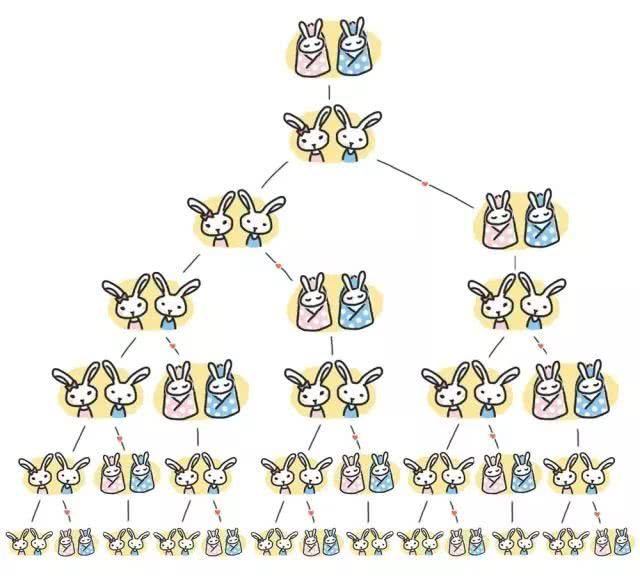
\includegraphics[scale=0.45]{img/C4/4-4/1.png}
\end{figure}

\begin{lstlisting}[language=Java]
import java.util.Scanner;

public class Fibonacci {
    public static void main(String[] args) {
        Scanner scanner = new Scanner(System.in);
        int n;
        int num1, num2, val;
        
        System.out.print("输入斐波那契数列长度:");
        n = scanner.nextInt();
        
        if(n == 1) {
            System.out.println("1");
        } else if(n == 2) {
            System.out.println("1, 1");
        } else {
            num1 = 1;
            num2 = 1;
            System.out.print("1, 1");
            for(int i = 3; i <= n; i++) {
                val = num1 + num2;
                System.out.print(", " + val);
                num1 = num2;
                num2 = val;
            }
            System.out.println();
        }
        scanner.close();
    }
}
\end{lstlisting}

\begin{tcolorbox}
	\mybox{运行结果}
	\begin{verbatim}
输入斐波那契数列长度:10
1, 1, 2, 3, 5, 8, 13, 21, 34, 55
    \end{verbatim}
\end{tcolorbox}

\subsection{嵌套循环}

循环也可以进行嵌套使用。 \\

\mybox{九九乘法表} \\

\begin{table}[H]
	\centering
	\setlength{\tabcolsep}{1.5mm}{
		\begin{tabular}{|c|c|c|c|c|c|c|c|c|}
			\hline
			1*1=1 & 1*2=2  & 1*3=3  & 1*4=4  & 1*5=5  & 1*6=6  & 1*7=7  & 1*8=8  & 1*9=9  \\
			\hline
			2*1=2 & 2*2=4  & 2*3=6  & 2*4=8  & 2*5=10 & 2*6=12 & 2*7=14 & 2*8=16 & 2*9=18 \\
			\hline
			3*1=3 & 3*2=6  & 3*3=9  & 3*4=12 & 3*5=15 & 3*6=18 & 3*7=21 & 3*8=24 & 3*9=27 \\
			\hline
			4*1=4 & 4*2=8  & 4*3=12 & 4*4=16 & 4*5=20 & 4*6=24 & 4*7=28 & 4*8=32 & 4*9=36 \\
			\hline
			5*1=5 & 5*2=10 & 5*3=15 & 5*4=20 & 5*5=25 & 5*6=30 & 5*7=35 & 5*8=40 & 5*9=45 \\
			\hline
			6*1=6 & 6*2=12 & 6*3=18 & 6*4=24 & 6*5=30 & 6*6=36 & 6*7=42 & 6*8=48 & 6*9=54 \\
			\hline
			7*1=7 & 7*2=14 & 7*3=21 & 7*4=28 & 7*5=35 & 7*6=42 & 7*7=49 & 7*8=56 & 7*9=63 \\
			\hline
			8*1=8 & 8*2=16 & 8*3=24 & 8*4=32 & 8*5=40 & 8*6=48 & 8*7=56 & 8*8=64 & 8*9=72 \\
			\hline
			9*1=9 & 9*2=18 & 9*3=27 & 9*4=36 & 9*5=45 & 9*6=54 & 9*7=63 & 9*8=72 & 9*9=81 \\
			\hline
		\end{tabular}
	}
	\caption{九九乘法表}
\end{table}

\begin{lstlisting}[language=Java]
public class MultiplicationTable {
    public static void main(String[] args) {
        for(int i = 1; i <= 9; i++) {
            for(int j = 1; j <= 9; j++) {
                System.out.print(
                    String.format("%d*%d=%d\t", i, j, i*j)
                );
            }
            System.out.println();
        }
    }
}
\end{lstlisting}

\vspace{0.5cm}

\mybox{输出图案}

\begin{lstlisting}
*
**
***
****
*****
\end{lstlisting}

\begin{lstlisting}[language=Java]
public class Stars {
    public static void main(String[] args) {
        for(int i = 1; i <= 5; i++) {
            for(int j = 1; j <= i; j++) {
                System.out.print("*");
            }
            System.out.println();
        }
    }
}
\end{lstlisting}

\newpage

\section{break or continue?}

\subsection{循环控制}

循环控制语句的作用是控制当前的循环结构是否继续向下执行,如果不进行控制,那么会根据既定的结构重复执行。如果有一些特殊的情况导致循环的执行中断,就称为循环的控制语句。循环控制语句的关键字有break和continue。 \\

break的作用是跳出当前循环,执行当前循环之后的语句。break只能跳出一层循环,如果是嵌套循环,那么需要按照嵌套的层次,逐步使用break来跳出。break语句只能在循环体内和switch语句内使用。 \\

continue的作用是跳过本轮循环,开始下一轮循环的条件判断。continue终止当前轮的循环过程,但它并不跳出循环。 \\

\mybox{break}

\begin{lstlisting}[language=Java]
public class Break {
    public static void main(String[] args) {
        for(int i = 1; i <= 10; i++) {
            if(i == 5) {
                break;
            }
            System.out.print(i + " ");
        }
    }
}
\end{lstlisting}

\begin{tcolorbox}
	\mybox{运行结果}
	\begin{verbatim}
1 2 3 4
    \end{verbatim}
\end{tcolorbox}

\vspace{0.5cm}

\mybox{continue}

\begin{lstlisting}[language=Java]
public class Continue {
    public static void main(String[] args) {
        for(int i = 1; i <= 10; i++) {
            if(i == 5) {
                continue;
            }
            System.out.print(i + " ");
        }
    }
}
\end{lstlisting}

\begin{tcolorbox}
	\mybox{运行结果}
	\begin{verbatim}
1 2 3 4 6 7 8 9 10
    \end{verbatim}
\end{tcolorbox}

\newpage